\vspace{\baselineskip}

\hspace{0,5cm}Notre expérience s'est divisée en deux axes. Le premier axe
consiste à déterminer comprendre et étudier le style d'écriture de Molière. Le
second axe consiste à déterminer les clusters de textes qui se ressemblent le
plus.

\hspace{0,5cm}Grâce à la bibliothèque \textbf{NLTK} et \textbf{WorldCloud}, nous
avons pu faire un nuage de mot pour le corpus de Molière. Un nuage de mots est
une manière de visualiser la fréquence des mots dans un corpus. Les mots
les plus fréquents sont présentés sous forme de nuage, où la taille du mot est
proportionnelle à sa fréquence. Cette représentation peut donner une vue
d'ensemble rapide des termes les plus courants dans le corpus de Molière. Pour
que l'analyse soit plus pertinente nous avons supprimé la prise en compte des
noms propres, qui sont uniques aux oeuvres.

\begin{figure}[htbp]
    \centering
    \includegraphics[width=15cm]{Ressources/nuage_sans_noms.png}
    \caption{Nuage de mots du corpus de Molière}
    \label{fig:images}
  \end{figure}

\vspace{\baselineskip}

\hspace{0,5cm}Grâce au nuage de mots, nous avions remarqué que le mot \textit{Monsieur}
revenait très souvent. Cette grande importance du mot \textit{Monsieur} dans le
nuage de mots révèle le vocabulaire et les règles d'écriture de l'époque.
\\Afin de mieux comprendre le style d'écriture de Molière, nous avons également
réaliser un histograme des mots les plus fréquents dans le corpus de Molière.
Pour rendre ce diagramme plus pertinent, nous avons décidé de ne pas prendre en
compte les noms de personnages mais également le mot \textit{Monsieur}.

\begin{figure}[htbp]
    \centering
    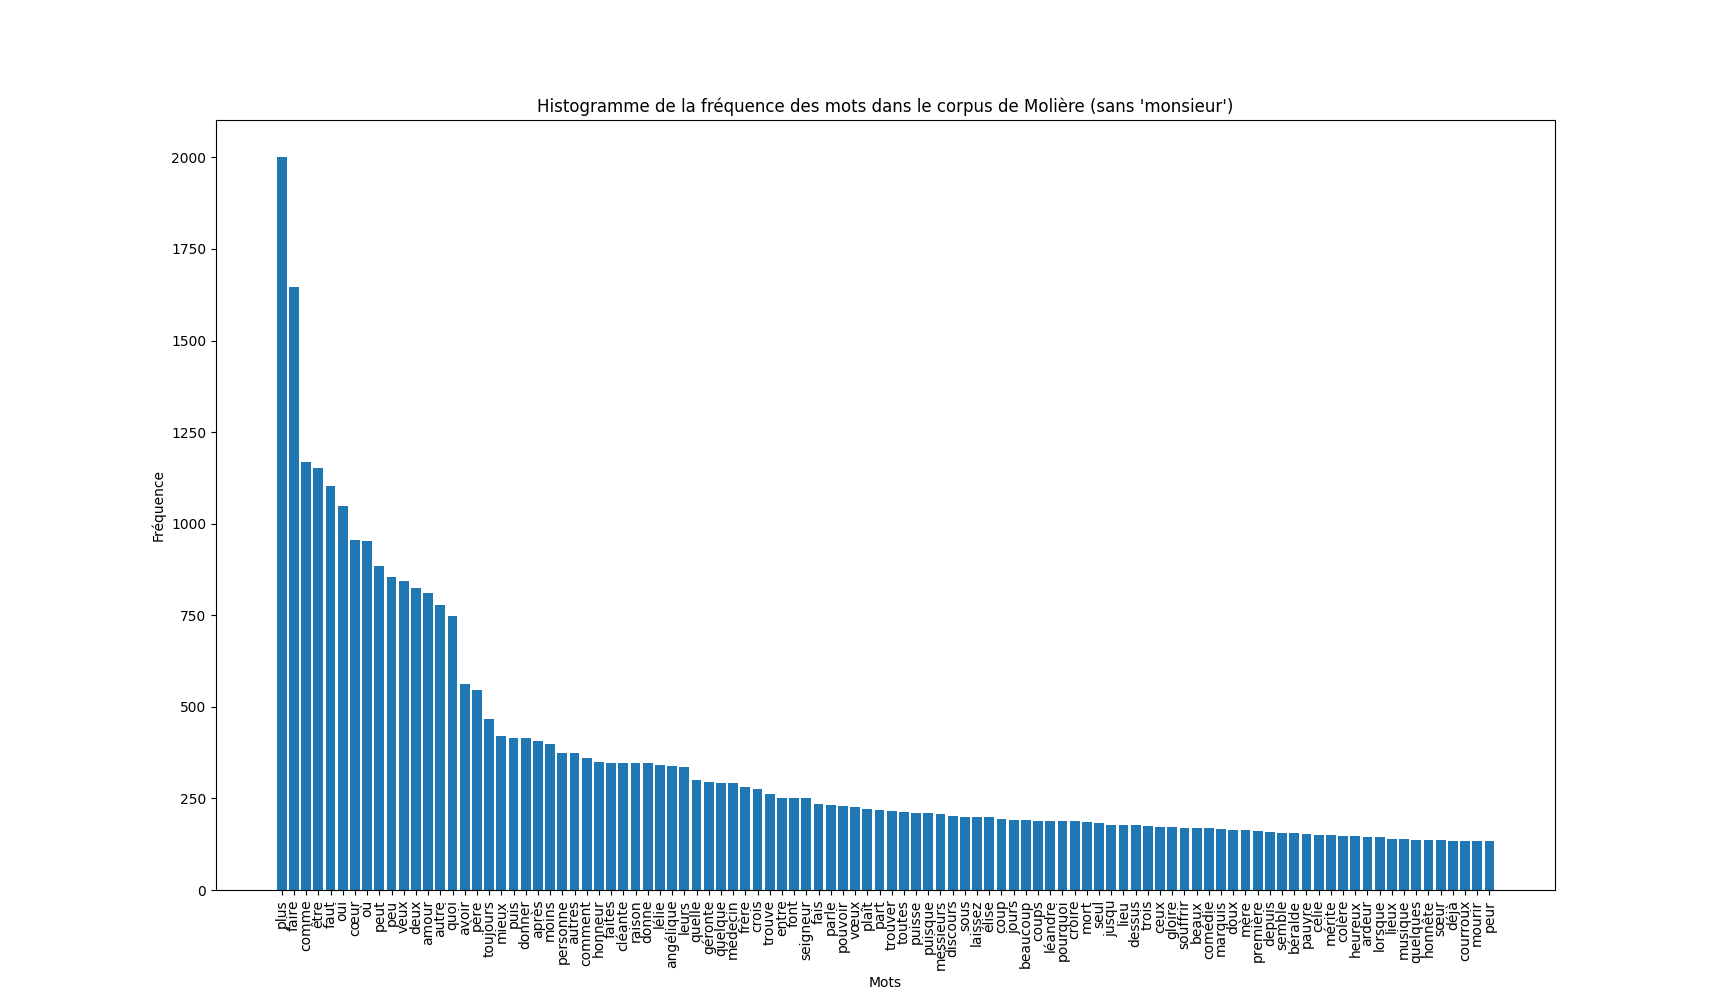
\includegraphics[width=13cm]{Ressources/diagr_sans_noms_mosn.png}
    \caption{Diagramme de mots du corpus de Molière sans le mot \textit{Monsieur}}
    \label{fig:images}
  \end{figure}

  \vspace{\baselineskip}

